%\documentclass[handout]{beamer}
\makeatletter\let\ifGm@compatii\relax\makeatother 
\documentclass[10pt]{beamer}
\usepackage[spanish]{babel}
\usepackage[ansinew]{inputenc}
\usepackage{amsmath}
\usepackage{enumerate}
\usepackage{exscale}
\usepackage{indentfirst}
\usepackage{latexsym}
\usepackage{proof}
\usepackage{color}
%\usepackage{subfig}

\usepackage{tikz}
\usetikzlibrary{backgrounds,fit,arrows} 

\usetheme{warsaw}

\newcommand{\ceil}[1]{\ensuremath{\left\lceil #1 \right\rceil}}
\newcommand{\floor}[1]{\ensuremath{\left\lfloor #1 \right\rfloor}}

\newcommand{\lpobjective}[2]{#1 \[ #2 \]}
\newcommand{\lprestriction}[3]{#1 \[ #2 \qquad #3 \]}
\newcommand{\lpineq}[2]{\[ #1 \qquad #2 \]}
\newcommand{\xor}{\veebar}

\newenvironment{centerblock}[1]{\begin{block}{#1}\center}{\end{block}}

\definecolor{briancolor}{rgb}{0.2,0.2,0.7}


\newcommand{\samplegraph}{
	\begin{tikzpicture}
		[n/.style= {thick,circle,draw=black}] 

		\node[n] (n0) at ( 0,0) {$v_0$}
		;

		\node[n] (n1) at ( 2,1) {$v_1$}
			edge [-]	(n0)
		;

		\node[n] (n2) at ( 2,3) {$v_2$}
			edge [-]	(n1)
		;
		
		\node[n] (n3) at ( 0,4) {$v_3$}
			edge [-]	(n1)
		;
		
		\node[n] (n4) at ( -2,3) {$v_4$}
			edge [-]	(n3)
			edge [-]	(n2)
		;
		
		\node[n] (n5) at ( -2,1) {$v_5$}
			edge [-]	(n2)
			edge [-]	(n4)
			edge [-]	(n0)
		;

	\end{tikzpicture} 
}

\newcommand{\samplecoloredgraph}{\begin{tikzpicture} 
		[n/.style= {thick,circle,draw=black}] 

		\node[n,fill=red!40] (n0) at ( 0,0) {$v_0$}
		;

		\node[n,fill=blue!40] (n1) at ( 2,1) {$v_1$}
			edge [-]	(n0)
		;

		\node[n,fill=red!40] (n2) at ( 2,3) {$v_2$}
			edge [-]	(n1)
		;
		
		\node[n,fill=red!40] (n3) at ( 0,4) {$v_3$}
			edge [-]	(n1)
		;
		
		\node[n,fill=blue!40] (n4) at ( -2,3) {$v_4$}
			edge [-]	(n3)
			edge [-]	(n2)
		;
		
		\node[n,fill=green!40] (n5) at ( -2,1) {$v_5$}
			edge [-]	(n2)
			edge [-]	(n4)
			edge [-]	(n0)
		;

	\end{tikzpicture} 
}

\newcommand{\samplepartitionedgraph}{
\begin{tikzpicture} 
		[n/.style= {minimum size=3mm,thick,circle,draw=black}] 

		\node[n] (n0) at ( 0,0) {$v_0$}
		;

		\node[n] (n1) at ( 2,1) {$v_1$}
			edge [-]	(n0)
		;

		\node[n] (n2) at ( 2,3) {$v_2$}
			edge [-]	(n1)
		;
		
		\node[n] (n3) at ( 0,4) {$v_3$}
			edge [-]	(n1)
		;
		
		\node[n] (n4) at ( -2,3) {$v_4$}
			edge [-]	(n3)
			edge [-]	(n2)
		;
		
		\node[n] (n5) at ( -2,1) {$v_5$}
			edge [-]	(n2)
			edge [-]	(n4)
			edge [-]	(n0)
		;
		
		\begin{pgfonlayer}{background} 
			\node [fill=black!5,fit=(n0) (n1)] {}; 
			\node [fill=blue!5,fit=(n2) (n3)] {}; 
			\node [fill=green!5,fit=(n4) (n5)] {}; 
		\end{pgfonlayer}

	\end{tikzpicture} }

\newcommand{\samplepartitionedcoloredgraph}{
\begin{tikzpicture} 
		[n/.style= {minimum size=3mm,thick,circle,draw=black}] 

		\node[n,fill=red!40] (n0) at ( 0,0) {$v_0$}
		;

		\node[n] (n1) at ( 2,1) {$v_1$}
			edge [-]	(n0)
		;

		\node[n,fill=green!40] (n2) at ( 2,3) {$v_2$}
			edge [-]	(n1)
		;
		
		\node[n] (n3) at ( 0,4) {$v_3$}
			edge [-]	(n1)
		;
		
		\node[n,fill=red!40] (n4) at ( -2,3) {$v_4$}
			edge [-]	(n3)
			edge [-]	(n2)
		;
		
		\node[n] (n5) at ( -2,1) {$v_5$}
			edge [-]	(n2)
			edge [-]	(n4)
			edge [-]	(n0)
		;
		
		\begin{pgfonlayer}{background} 
			\node [fill=black!5,fit=(n0) (n1)] {}; 
			\node [fill=blue!5,fit=(n2) (n3)] {}; 
			\node [fill=green!5,fit=(n4) (n5)] {}; 
		\end{pgfonlayer}

	\end{tikzpicture} 
}

\newcommand{\samplenetwork}
{\begin{tikzpicture} 
		[bend angle=40,
		n/.style={font=\tiny,minimum size=2mm,thick,circle,draw=black!75,fill=black!25}] 
		
		\node[n] (n0) at ( 0,0) {$s_1$}; 
		
		\node[n] (n1) at ( 0,1) {}
			edge [-]	(n0)
		;

		\node[n] (n2) at ( 1,2) {}
			edge [-]	(n1)
		;
		
		\node[n] (n4) at ( 1,0) {}
			edge [-]	(n0)
		;
		
		\node[n] (n5) at ( 2,1) {}
			edge [-]	(n4)
		;
		
		\node[n] (n3) at ( 2,2) {$t_1$}
			edge [-]	(n2)
			edge [-]	(n5)
			edge [<-, draw=black!50] node[auto] {} 	(n0)
			
		;
		
		\node[n] (n6) at ( 1,-1) {$s_2$}
			edge [-]	(n4)
		;
		
		\node[n] (n7) at ( 3,1) {$t_2$}
			edge [-]	(n5)
			edge [<-, draw=black!50] node[auto] {} 	(n6)
			
		;
		
		\node[n] (n8) at ( 2,-1) {}
			edge [-]	(n6)
		;

		\node[n] (n9) at ( 3,0) {}
			edge [-]	(n8)
			edge [-]	(n7)
		;
			\end{tikzpicture} 
}

\newcommand{\samplenetworkroutes}
{
\begin{tikzpicture} 
		[bend angle=40,
		n/.style= {font=\tiny,minimum size=3mm,thick,circle,draw=black!75,fill=black!25}] 
		
		\node[n] (n0) at ( 0,0) {$s_1$}; 
		
		\node[n] (n1) at ( 0,1) {}
			edge [-]	(n0)
		;

		\node[n] (n2) at ( 1,2) {}
			edge [-]	(n1)
		;
		
		\node[n] (n4) at ( 1,0) {}
			edge [-]	(n0)
		;
		
		\node[n] (n5) at ( 2,1) {}
			edge [-]	(n4)
		;
		
		\node[n] (n3) at ( 2,2) {$t_1$}
			edge [-]	(n2)
			edge [-]	(n5)
			edge [<-, bend right, draw=black!50] node[auto,font=\tiny] {$R_1$} 	(n0)
			edge [<-, bend left, draw=black!50] node[auto,swap,font=\tiny] {$R_2$} (n0)
		;
		
		\node[n] (n6) at ( 1,-1) {$s_2$}
			edge [-]	(n4)
		;
		
		\node[n] (n7) at ( 3,1) {$t_2$}
			edge [-]	(n5)
			edge [<-, bend right, draw=black!50] node[auto,font=\tiny] {$R_3$}  (n6)
			edge [<-, bend left, draw=black!50]	node[auto,swap,font=\tiny] {$R_4$} (n6) 
		;
		
		\node[n] (n8) at ( 2,-1) {}
			edge [-]	(n6)
		;

		\node[n] (n9) at ( 3,0) {}
			edge [-]	(n8)
			edge [-]	(n7)
		;
		
	\end{tikzpicture} 
	}
	
\newcommand{\networkpcpgraph}
{
\begin{tikzpicture} 
			[n/.style= {font=\tiny,minimum size=1mm,thick,circle,draw=black!75}] 

			\node[n,fill=black!25] (n0) at ( 0,0) {$R_1$}; 

			\node[n,fill=black!25] (n1) at ( 0,1) {$R_2$};

			\node[n,fill=black!25] (n2) at ( 3,0) {$R_3$}
				edge [-]	(n1)
			;

			\node[n,fill=black!25] (n3) at ( 3,1) {$R_4$};

			\begin{pgfonlayer}{background} 
				\node [font=\tiny,fill=black!10,circle,fit=(n0) (n1),label=170:$s_1 \rightarrow t_1$] {}; 
				\node [font=\tiny,fill=black!10,circle,fit=(n2) (n3),label=350:$s_2 \rightarrow t_2$] {}; 
			\end{pgfonlayer}

		\end{tikzpicture} 
}

\newcommand{\networkpcpcoloredgraph}
{
\begin{tikzpicture} 
			[n/.style= {font=\tiny,minimum size=1mm,thick,circle,draw=black!75}] 

			\node[n,fill=blue!75] (n0) at ( 0,0) {$R_1$}; 

			\node[n,fill=black!25] (n1) at ( 0,1) {$R_2$};

			\node[n,fill=black!25] (n2) at ( 3,0) {$R_3$}
				edge [-]	(n1)
			;

			\node[n,fill=blue!75] (n3) at ( 3,1) {$R_4$};

				\begin{pgfonlayer}{background} 
					\node [font=\tiny,fill=black!10,circle,fit=(n0) (n1),label=170:$s_1 \rightarrow t_1$] {}; 
					\node [font=\tiny,fill=black!10,circle,fit=(n2) (n3),label=350:$s_2 \rightarrow t_2$] {}; 
				\end{pgfonlayer}

		\end{tikzpicture} 
}

\newcommand{\solvednetwork}
{
\begin{tikzpicture} 
		[bend angle=40,
		n/.style= {font=\tiny,minimum size=3mm,thick,circle,draw=black!75,fill=black!25}] 
		
		\node[n] (n0) at ( 0,0) {$s_1$}; 
		
		\node[n] (n1) at ( 0,1) {}
			edge [-]	(n0)
		;

		\node[n] (n2) at ( 1,2) {}
			edge [-]	(n1)
		;
		
			\node[n] (n4) at ( 1,0) {}
			edge [-]	(n0)
		;
		
		\node[n] (n5) at ( 2,1) {}
			edge [-]	(n4)
		;
		
		\node[n] (n3) at ( 2,2) {$t_1$}
			edge [-]	(n2)
			edge [-]	(n5)
			edge [<-, bend right, draw=blue!100] node[font=\tiny,auto] {\textcolor{blue!100}{$R_1$}} 	(n0)
			edge [<-, bend left, draw=black!10] node[font=\tiny,auto,swap] {\textcolor{black!10}{$R_2$}} (n0)
		;
		
		\node[n] (n6) at ( 1,-1) {$s_2$}
			edge [-]	(n4)
		;
		
		\node[n] (n7) at ( 3,1) {$t_2$}
			edge [-]	(n5)
			edge [<-, bend right, draw=black!10] node[font=\tiny,auto] {\textcolor{black!10}{$R_3$}}  (n6)
			edge [<-, bend left, draw=blue!100]	node[font=\tiny,auto,swap] {\textcolor{blue!100}{$R_4$}} (n6) 
		;
		
		\node[n] (n8) at ( 2,-1) {}
			edge [-]	(n6)
		;

		\node[n] (n9) at ( 3,0) {}
			edge [-]	(n8)
			edge [-]	(n7)
		;
		
	\end{tikzpicture} 
}

\newcommand{\lpsample}{
\begin{tikzpicture}
[scale=3,line cap=round
% Styles
axes/.style=,
important line/.style={very thick},
information text/.style={rounded corners,fill=red!10,inner sep=1ex}]
% Local definitions
\def\costhirty{0.8660256}
% Colors
\colorlet{anglecolor}{green!50!black}
\colorlet{sincolor}{red}
\colorlet{tancolor}{orange!80!black}
\colorlet{coscolor}{blue}
% The graphic
\draw[help lines,step=0.5cm] (-1.4,-1.4) grid (1.4,1.4);
\draw (0,0) circle (1cm);
\begin{scope}[axes]
\draw[->] (-1.5,0) -- (1.5,0) node[right] {$x$} coordinate(x axis);
\draw[->] (0,-1.5) -- (0,1.5) node[above] {$y$} coordinate(y axis);
\foreach \x/\xtext in {-1, -.5/-\frac{1}{2}, 1}
\draw[xshift=\x cm] (0pt,1pt) -- (0pt,-1pt) node[below,fill=white] {$\xtext$};
\foreach \y/\ytext in {-1, -.5/-\frac{1}{2}, .5/\frac{1}{2}, 1}
\draw[yshift=\y cm] (1pt,0pt) -- (-1pt,0pt) node[left,fill=white] {$\ytext$};
\end{scope}
\filldraw[fill=green!20,draw=anglecolor] (0,0) -- (3mm,0pt) arc(0:30:3mm);
\draw (15:2mm) node[anglecolor] {$\alpha$};
\draw[important line,sincolor]
(30:1cm) -- node[left=1pt,fill=white] {$\sin \alpha$} (30:1cm |- x axis);
\draw[important line,coscolor]
(30:1cm |- x axis) -- node[below=2pt,fill=white] {$\cos \alpha$} (0,0);
\draw[important line,tancolor] (1,0) -- node[right=1pt,fill=white] {
$\displaystyle \tan \alpha \color{black}=
\frac{{\color{sincolor}\sin \alpha}}{\color{coscolor}\cos \alpha}$}
(intersection of 0,0--30:1cm and 1,0--1,1) coordinate (t);
\draw (0,0) -- (t);
\draw[xshift=1.85cm]
node[right,text width=6cm,information text]
{
The {\color{anglecolor} angle $\alpha$} is $30^\circ$ in the
example ($\pi/6$ in radians). The {\color{sincolor}sine of
$\alpha$}, which is the height of the red line, is
\[
{\color{sincolor} \sin \alpha} = 1/2.
\]
By the Theorem of Pythagoras ...
};
\end{tikzpicture}
36
}
%\includeonly{resolucion}

\begin{document}

\begin{frame}
\titlepage
\end{frame}

\setlength{\parskip}{10pt plus 1pt minus 1pt}
\section{Introducci\'on}
\subsection{Grafos}

\begin{frame}
\frametitle{Grafos}

Un grafo $G$ se define como un par $V,E$ donde $V$ es un conjunto de nodos, unidos por los ejes del conjunto $E$.

\vspace{11pt}

\begin{figure}[h]
	\centering	
	\samplegraph
\end{figure}

\end{frame} 

\begin{frame}
\frametitle{Coloreo}

El problema de coloreo consiste en asignar un \textbf{color} a cada nodo de manera tal que dos nodos adyacentes tengan colores distintos. Se busca minimizar la cantidad de colores a utilizar.

\begin{figure}[h]
	\centering	
	\samplecoloredgraph
\end{figure}

\end{frame}	

\begin{frame}
\frametitle{Coloreo}

Pintando el mapa de sudam�rica...

\begin{figure}[h]
	\centering
	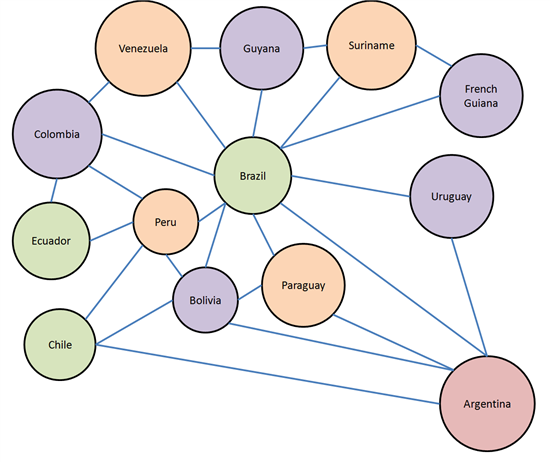
\includegraphics[scale=0.5]{../imgs/southamerica.png}
\end{figure}


\end{frame}


\begin{frame}
\frametitle{Grafos particionados}

Un grafo \textbf{particionado} es un grafo en el que el conjunto de nodos se encuentra dividido en particiones $P_0, \ldots,P_q$.

\vspace{21pt}

\begin{figure}[h]
	\centering	
	\samplepartitionedgraph
\end{figure}

\end{frame}

\begin{frame}
\frametitle{Coloreo particionado}

El problema de coloreo \textbf{particionado} consiste en, dado un grafo particionado, asignar un \textbf{color} a un solo nodo por particion, de manera tal que dos nodos adyacentes no usen colores iguales. Se busca minimizar la cantidad de colores a utilizar.

\begin{figure}[h]
	\centering	
	\samplepartitionedcoloredgraph
\end{figure}

\end{frame}

\subsection{Motivaci�n}

\begin{frame} 
\frametitle{Redes WDM}

Wavelength-division multiplexing (WDM) permite multiplexar distintas se�ales �pticas sobre un mismo enlace f�sico utilizando distintas frecuencias para cada uno.

\begin{figure}[h]
	\centering
	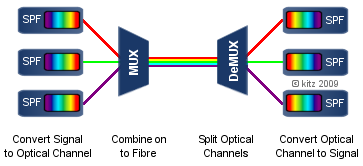
\includegraphics[scale=0.5]{../imgs/wdm.png}
\end{figure}

Se tiene una red compuesta por nodos en la que las conexiones entre ellos utilizan esta tecnolog�a. 

\end{frame} 

\begin{frame} 
\frametitle{Problema}

Se tiene un conjunto de pedidos de conexiones entre nodos, donde cada conexi�n debe usar una �nica frecuencia a lo largo de todo el camino, y si dos conexiones comparten algun enlace f�sico deben usar frecuencias distintas.

El objetivo es determinar un conjunto de rutas tal que se minimice la cantidad de frecuencias distintas usadas.

\begin{figure}[h]
	\centering
	\samplenetwork
\end{figure}

\end{frame} 

\begin{frame} 
\frametitle{Resoluci�n en dos partes}

Li y Sinha propusieron una soluci�n en dos partes para este problema:
\begin{enumerate}
\item{Generar un conjunto de rutas posibles entre cada par de nodos a conectar}
\item{Elegir una ruta de cada conjunto de manera tal que se minimice la cantidad de frecuencias necesarias}
\end{enumerate}

\end{frame} 

\begin{frame} 
\frametitle{Generaci�n de rutas}

Mediante una heur�stica, se genera una cierta cantidad de caminos distintos entre cada par de nodos que se desean conectar. Pueden usarse criterios de camino m�nimo o de maximum edge disjoint path.

\begin{figure}[h]
	\centering
	\samplenetworkroutes
\end{figure}

\end{frame} 

\begin{frame} 
\frametitle{Asignaci�n de frecuencias}

El siguiente paso es elegir una ruta entre cada par de nodos y asignarle una frecuencia, de manera tal que dos rutas distintas con la misma frecuencia no compartan ning�n enlace.

Esto puede modelarse como un problema de coloreo particionado:
\begin{itemize}
\item{Los nodos representan las rutas}
\item{Las rutas est�n agrupadas en particiones seg�n qu� conexi�n satisfacen}
\item{Los ejes indican que las rutas comparten al menos un enlace y no pueden compartir frecuencia}
\item{Las frecuencias se modelan mediante los colores}
\end{itemize}

\end{frame} 

\begin{frame} 
\frametitle{Asignaci�n de frecuencias}

Nuestro ejemplo puede resolverse usando una �nica frecuencia...

\begin{figure}[h]
		\centering	
		\alt<1>{\networkpcpgraph}{\networkpcpcoloredgraph}
\end{figure}

\begin{figure}[h]
	\centering
	\alt<1>{\samplenetworkroutes}{\solvednetwork}
\end{figure}

\uncover<2>{}

\end{frame}
\section{Modelo}

\subsection{Modelo inicial de coloreo}
\begin{frame} 
\frametitle{Modelo de coloreo}

Definimos las siguientes variables binarias:

\begin{itemize}
\item{$x_{ij}$ es verdadera sii el v�rtice $i$ es coloreado con el color $j$}
\item{$w_{j}$ es verdadera sii el color $j$ fue usado}
\end{itemize}

\uncover<2>{
\lpobjective{Buscamos minimizar la cantidad de colores distintos usados}
{\min \sum_{j \in C} w_{j}}
}

\end{frame} 

\begin{frame} 
\frametitle{Modelo de coloreo}

Agregamos las restricciones de coloreo:

\begin{itemize}
\item<2->{
\lprestriction{La variable $w_j$ es verdadera sii alg�n v�rtice usa el color $j$}
{x_{ij} \leq w_j}{\forall j \in C, \forall i \in V}
}

\item<3->{
\lprestriction{Dos vecinos no pueden usar el mismo color}
{x_{ij} + x_{kj} \leq 1}{\forall j \in C, \forall (i,k) \in E}
}

\item<4->{
\lprestriction{Cada \only<4>{v�rtice}\alert<5>{\only<5>{partici�n}} tiene exactamente un color asignado}
{\uncover<5>{\sum _{x_i \in p}} \sum_{j \in C} x_{ij} = 1}{\forall i \in V \uncover<5>{, p \in P}}
}
\end{itemize}

\end{frame} 

\begin{frame}
\frametitle{Modelo de coloreo}

Con esto ya tenemos una formulaci�n b�sica del problema que podemos resolver con un algoritmo de branch and cut. Pero podemos reforzar la formulaci�n para mejorar los tiempos de resoluci�n del algoritmo:

\begin{itemize}
\item{expresando las restricciones de adyacencia de otras maneras}
\item{agregando restricciones de eliminacion de simetr�a}
\item{agregando otras desigualdades v�lidas}
\end{itemize}

\end{frame} 

\subsection{Reforzando el modelo}

\begin{frame}
\frametitle{Restricciones de adyacencia}

\begin{itemize}
\item{
\lprestriction{Dado un nodo $i_0$, por cada partici�n vecina, o bien $i_0$ usa el color $j$, o a lo sumo uno de sus vecinos por partici�n puede usarlo.}
{\sum_{i \in P_k \cap N(i_0)} x_{ij} + x_{i_0j} \leq w_j}{\forall j \in C, \; \forall P_k \in P, \; \forall i_0 \in V }
\begin{figure}[h]
\centering
\uncover<2->{\alt<2>{\adjsrestrictionpartone}{\adjsrestrictionparttwo}}
\end{figure}
}
\end{itemize}

\uncover<4>{
\begin{centerblock}{}
Estas restricciones arrojaron los mejores resultados para grafos de alta densidad.
\end{centerblock}
}

\end{frame} 

\begin{frame}
\frametitle{Restricciones de adyacencia}

\begin{itemize}
\item{
\lprestriction{Generalizamos las anteriores pidiendo o bien un nodo $i_0$ usa el color $j$, o bien a lo sumo \alert<3->{$r$} de sus vecinos lo utilizan.}
{\sum_{i \in N(i_0)} x_{i_0j} + \alert<3->{r} * x_{i_0j} \leq \alert<3->{r} * w_j}{\forall j \in C, \; \forall i_0 \in V}
\begin{figure}[h]
\centering
\uncover<2->{\adjsrestrictionneighbours}
\end{figure}
}
\end{itemize}

\uncover<4>{
\begin{centerblock}{}
Estas restricciones arrojaron los mejores resultados para grafos de baja densidad.
\end{centerblock}
}

\end{frame} 

\subsection{Eliminaci�n de simetr�a}
\begin{frame}{Eliminaci�n de simetr�a}

Un problema inherente a coloreo, que se traduce al modelo, es que admite muchas soluciones sim�tricas para un mismo grafo:

\begin{center}
	\samplepartitionedcoloredgraphA
	\samplepartitionedcoloredgraphB
\\
\vskip 4pt
	\samplepartitionedcoloredgraphC
	\samplepartitionedcoloredgraphD
\end{center}

\end{frame} 

\begin{frame}{Eliminaci�n de simetr�a}

Buscamos agregar restricciones al modelo que eliminen soluciones sim�tricas:

\begin{itemize}
\item<2->{
\lprestriction{No se permite usar un color hasta que no se hayan usado todos los anteriores}
{w_j \geq w_{j+1}}{\forall 1 \leq j < c }
}
\end{itemize}

\uncover<3>{Esta restricci�n asegura que s�lo se usen los primeros colores, pero permite soluciones simetr�cas que usan el mismo conjunto de colores.}

\end{frame}

\begin{frame}{Eliminaci�n de simetr�a}

\begin{itemize}
\item{
\lprestriction{La cantidad de nodos coloreados con un color $j_0+1$ no puede ser mayor que la cantidad coloreada con $j_0$.}
{\sum_{i \in V} x_{ij} \geq \sum_{i \in V} x_{ij+1}}{\forall 1 \leq j < c }
}
\end{itemize}

\uncover<2>{Elimina muchas soluciones sim�tricas, pero a�n permite intercambiar colores entre aquellos usados por la misma cantidad de nodos.}

\end{frame}

\begin{frame}{Eliminaci�n de simetr�a}

\begin{itemize}
\item{
\lprestriction{Asignamos el color de menor �ndice al conjunto de nodos que tenga la partici�n de menor �ndice}
{x_{ij} \leq \sum_{l = j-1}^{k-1} \sum_{u \in P_l} x_{uj-1}}{\forall 1 < k \leq q, \; \forall i \in P_k, \; \forall 1 < j \leq k}
}
\item<2->{
\lprestriction{Ninguna partici�n puede estar coloreada con un color de etiqueta mayor a su �ndice}
{x_{ij} = 0}{\forall j > p(i) + 1}
}
\end{itemize}

\uncover<3>{
\begin{centerblock}{}
Este par de restricciones es el que mejores resultados arroj� en el algoritmo implementado.
\end{centerblock}
}

\end{frame}


\begin{frame}
\frametitle{Desigualdades v�lidas en el modelo}

\begin{itemize}

\item{
\lprestriction{Ning�n v�rtice puede usar un color de etiqueta mayor a la cantidad de colores usados.}
{\sum_{j \in C} j x_{ij} \leq \sum_{j \in C} w_j}
{\forall i \in V}
}


\item<2>{
\lprestriction{{\alert{Ninguna partici�n}} puede usar un color de etiqueta mayor a la cantidad de colores usados.}
{\sum_{j \in C} \sum_{i \in P_k} j x_{ij} \leq \sum_{j \in C} w_j}
{\forall P_k \in P}
}

\end{itemize}

\end{frame} 


\section{Algoritmo}
\begin{frame}{Resoluci�n}

Una vez fijado el modelo, una manera de resolver un problema de programaci�n lineal entera consiste en aplicar un algoritmo de \textit{branch and cut}, el cual es una combinaci�n de las t�cnicas de \alert<2>{planos de corte} y de \alert<3>{branch and bound}.
\vskip 5pt
\uncover<2->{La primera se basa en resolver el problema de programaci�n lineal \textbf{sin} las restricciones de integralidad, eliminar la solucci�n fraccionaria con alg�n criterio, y repetir el proceso hasta llegar a una soluci�n �ptima entera.}
\vskip 5pt
\uncover<3->{La segunda subdivide el problema sucesivamente en otros m�s peque�os, eliminando ciertas soluciones fraccionarias, y manteniendo durante el recorrido del �rbol generado una cota superior y otra inferior para el �ptimo buscado.}

\end{frame} 

\begin{frame}{Componentes}

Un algoritmo de branch and cut consta entonces, de los siguientes componentes:

\begin{itemize}
\item<2->{\textbf{Algoritmos de separaci�n}, para remover soluciones fraccionales aplicando planos de corte construidos a partir de desigualdades v�lidas}
\item<3->{\textbf{Estrategias de branching}, para decidir con qu� criterio se subdivide el problema a cada nodo del �rbol}
\item<4->{\textbf{Heur�sticas inicial y primal}, para contar con soluciones enteras factibles durante el recorrido del �rbol, que act�an como cotas superiores para el �ptimo.}
\end{itemize}

\end{frame} 

\subsection{Planos de corte}

\begin{frame} 
\frametitle{Desigualdades v�lidas para PCP}

\begin{itemize}

\item{En una clique extendida, cada nodo debe tener un color distinto.
\lpineq{\sum_{i \in K} x_{ij_0} \leq w_{j_0}}{\forall j_0 \in C}
\extclique
\uncover<2>{Usamos un algoritmo goloso basado en los valores de las variables y los grados de los nodos para construir los planos de corte correspondientes.}
}

\end{itemize}

\end{frame} 


\begin{frame} 
\frametitle{Desigualdades v�lidas para PCP}

\begin{itemize}

\item{Una partici�n no puede colorearse con el color $j_0$ a menos que todos los anteriores ya hayan sido usados.
\lpineq{\sum_{i \in p_0}\sum_{j \geq j_0} x_{ij} \leq w_{j_0}}{\forall p_0 \in P, j_0 \in C}}

\uncover<2->{
Hay solamente $|P| \times |C|$, con lo que pueden resolverse mediante simple enumeraci�n.
}

\end{itemize}

\end{frame} 

\begin{frame} 
\frametitle{Desigualdades v�lidas para PCP}

\begin{itemize}

\item{Dado un maximum component independent set $I$ de tama�o $\alpha$ tal que cada nodo est� en una partici�n distinta, a lo sumo $\alpha$ nodos pueden tener el mismo color.
\lpineq{\sum _{i \in I} x_{ij_0} \leq \alpha w_{j_0}}{\forall j_0 \in C}

\uncover<2->{
Especializamos esta desigualdad tomando subgrafos cuyos conjunto independientes m�ximos son f�ciles de calcular.

\begin{itemize}
\item{Component paths}
\item{Component holes}
\end{itemize}
}

\uncover<3->{Nuevamente usamos un algoritmo goloso para construir estos planos de corte, acotando la cantidad de veces que cada nodo y cada eje puede ser visitado.}}

\end{itemize}
\end{frame} 

\begin{frame} 
\frametitle{Desigualdades v�lidas para PCP}

\begin{itemize}

\item Dado un grafo, definimos su \textit{grafo de particiones} como un grafo que tiene un nodo por cada partici�n del original, y dos nodos son adyacentes sii todos los nodos de las dos particiones eran adyacentes entre s�:
\uncover<2->{
	\alt<2>
	{\togprime}
	{\gprime}
}

\uncover<4->{Las desigualdades de conjunto independiente se pueden aplicar sobre el grafo de particiones y llevarse al grafo original.}
\vfill
\end{itemize}

\end{frame} 

\begin{frame} 
\frametitle{Planos de corte}

Analizamos el gap en grafos de distinta densidad al aplicar distintas familias de corte sobre los ya provistos por \textsc{cplex} en un algoritmo de planos de corte:

\includechart{chartcuts.png}

\end{frame} 

\subsection{Estrategia de branching}

\begin{frame}{Estrategia de Branching}

Lo siguiente es definir una estrategia de branching, que determina c�mo generar los subproblemas a partir de un nodo del �rbol.
\vskip 3pt
\uncover<2->{Las estrategias t�picas son tomar la variable con valor m�s fraccionario o menos fraccionario en la soluci�n de la relajaci�n, y forzar a que tome valor $0$ o $1$ en cada hijo.
\begin{figure}[h]
	\centering
	\branchingtree
\end{figure}
}
\end{frame} 

\begin{frame}{Estrategia de Branching en PCP}

En PCP usamos como criterio de branching seleccionar un nodo de una partici�n sin colorear y asignarle un color distinto entre todos los posibles en los subproblemas:

\begin{figure}[h]
	\centering
	\pcpbranchingtree
\end{figure}

\uncover<2->{El nodo elegido a colorear es el que tiene mayor grado de saturaci�n, es decir, distintos colores usados para sus vecinos.}

\end{frame} 

\begin{frame}{Estrategia de Branching en PCP}

Comparando contra las otras estrategias en grafos de distinta densidad en un branch and bound:

\includechart{chartbranchingstrategy.png}

\end{frame} 

\subsection{Heur�sticas Primal e Inicial}

\begin{frame}{Heur�sticas}

La heur�stica primal se utiliza para generar soluciones enteras a lo largo del algoritmo, que act�an como cota superior para el �ptimo.

Una heur�stica usual consiste en redondear las variables de acuerdo a su valor fraccionario en la relajaci�n para llegar a una soluci�n entera.

\uncover<2>{Nosotros adaptamos algoritmos existentes de coloreo a este problema para utilizar como heur�sticas.}

\end{frame}

\begin{frame}{Algoritmos de enumeraci�n}

En coloreo, un algoritmo de enumeraci�n recorre posibles coloreos, eliminando gran cantidad de soluciones sim�tricas y podando aquellos que no logran un valor mejor al alcanzado hasta el momento.

En cada iteraci�n, se elige un nodo y se intenta colorearlo con los colores disponibles.

\uncover<2->{Distintos criterios para elegir el nodo a colorear dan lugar a distintos algoritmos:
\begin{itemize}
\item{Mayor grado del nodo}
\item{Menor grado del nodo}
\alert<3>{\item{Mayor grado de saturaci�n}}
\end{itemize}
}

\end{frame}

\begin{frame}{DSatur}

La variante que utiliza el mayor grado de saturaci�n, \textsc{DSatur}, es una de las que mejores tiempos logra. 

\uncover<2->{Si bien es un algoritmo exacto, limitamos su ejecuci�n a una determinada cantidad de tiempo para usarlo como heur�stica, pues arroja soluciones muy buenas en poco tiempo.}

\uncover<3->{Puede generalizarse para coloreo particionado seg�n distintos criterios:
\begin{itemize}
\alert<4>{\item{\textbf{Nodo m�s sencillo:} de cada partici�n sin colorear, se toma el nodo de menor grado de saturaci�n, luego se elige entre ellos el de mayor grado.}}
\alert<5>{\item{\textbf{Partici�n m�s dif�cil:} se determina cu�l es la partici�n a�n no coloreada m�s dif�cil seg�n distintos criterios, y de ella se elige el nodo de menor grado de saturaci�n.}}
\end{itemize}
}

\end{frame}

\begin{frame}{DSatur Particionado}

Comparamos estos criterios en corridas de un minuto sobre grafos de distinta densidad:
\includechart{chartdsatur.png}

\end{frame} 

\begin{frame}{Heur�stica inicial}

Teniendo definida la variante de DSatur a utilizar, la aplicamos como heur�stica inicial, ejecutando por 5 segundos.
\vskip 3pt
Esto no s�lo provee una soluci�n inicial para el algoritmo, que act�a como cota superior desde el principio del �rbol, sino que tambi�n acota considerablemente la cantidad de variables y restricciones. 
\vskip 3pt
\uncover<2->{
Sea $\alert<3>{\chi_0}$ la soluci�n de la heur�stica inicial,
\begin{align*}
x_{ij} \quad &1 \leq i \leq |V|,\; 1 \leq j \leq \alt<2>{|P|}{\alert{\chi_0}} \\
w_{j} \quad &1 \leq j \leq \alt<2>{|P|}{\alert{\chi_0}}
\end{align*}}
\uncover<3->{Por cada color que no se utilice en la soluci�n inicial, se tienen $|V|+1$ variables menos.}

\end{frame}

\begin{frame}{Heur�stica primal}

Dada una soluci�n fraccionaria, fijamos en $1$ aquellas variables $x_{ij}$ mayores a determinado valor. A partir de ese coloreo parcial, utilizamos DSatur para construir una soluci�n entera v�lida.

\uncover<2->{
\begin{block}{}
Si bien la heur�stica primal funciona correctamente, la inicial arroja un resultado demasiado cerca del �ptimo, lo cual hace que la heur�stica primal sea incapaz de mejorar el resultado inicial en la mayor�a de los casos. S�lo en grafos muy densos logra una mejora respecto de la soluci�n inicial.
\end{block}
}

\end{frame}


\begin{frame}
\frametitle{Branch and Bound}

Otro componente del branch and bound es la \textit{heur�stica primal}: consiste en derivar una soluci�n entera a partir de un �ptimo de la relajaci�n.

Un esquema t�pico consiste en tomar las variables con valor fraccionario y redondearlas al valor entero m�s cercano.

\uncover<2->{En PCP fijamos las variables con valor suficientemente grande y corremos un algoritmo de coloreo secuencial basado en el grado de saturaci�n de los nodos}.

\end{frame}

\begin{frame}
\frametitle{Branch and Cut}

Un algoritmo de \textit{branch and cut} es una combinaci�n de branch and bound y planos de corte.

Sobre un esquema de branch and bound, se ejecutan planos de corte cada cierta cantidad de nodos para eliminar a�n m�s soluciones fraccionarias.

\uncover<2->{Esta t�cnica es la que suele dar los mejores resultados pr�cticos a la hora de resolver un problema de estas caracter�sticas.}

\end{frame}

\end{document}


